\documentclass[12pt]{article}
%
\usepackage{graphicx}
\usepackage[margin=0.85in,footskip=0.2in]{geometry}%big footskip brings number down, small footskip br
\usepackage{amsmath}
\usepackage{amssymb}
\usepackage[T1]{fontenc}
\usepackage{listings}
\usepackage{bm}
\usepackage{hyperref}
\usepackage{setspace}
\usepackage[usenames]{color}
\usepackage[utf8]{inputenc}
\usepackage{wrapfig}
\usepackage{relsize}
\usepackage{psfrag}
\usepackage{dsfont}

%
%
\usepackage{titlesec}
\titlespacing*{\section}{0pt}{0.25\baselineskip}{0.25\baselineskip}
\titlespacing*{\subsection}{0pt}{0.5\baselineskip}{0.5\baselineskip}
%\titleformat*{\section}{\LARGE \bfseries}
\titleformat*{\section}{\large \bfseries}

%
\begin{document}

\pagenumbering{gobble}
%
\title{Improving Catch Estimation Methods in Sparsely Sampled Mixed-Stock Fisheries.}
\author{Nick Grunloh$^\text{a}$, Edward Dick$^\text{b}$, Don Pearson$^\text{b}$, John Field$^\text{b}$, Marc Mangel$^\text{a,c}$}
\date{August 15, 2017}
%
\maketitle
%
\begin{abstract}
%
Effective management of exploited fish populations requires accurate
estimates of commercial fisheries catches to inform monitoring and
assessment efforts. In California, the high degree of heterogeneity in
the species composition of many groundfish fisheries, particularly those
targeting rockfish (genus $Sebastes$), leads to challenges in sampling all
potential strata, or species, adequately. Limited resources and
increasingly complex stratification of the sampling system inevitably
leads to gaps in sample data. In the presence of sampling gaps, ad-hoc
species composition point estimation is currently obtained according to
historically derived ``data borrowing'' (imputation) protocols which do
not allow for uncertainty estimation or forecasting. In order to move
from the current ad-hoc ``data-borrowing'' point estimators, we have
constructed Bayesian hierarchical models to estimate species
compositions, complete with accurate measures of uncertainty, as well as
theoretically sound out-of-sample predictions. Furthermore, we introduce
a computational method for discovering consistent ``borrowing''
strategies across over-stratified data. Our modeling approach, along
with a computationally robust system of inference and model exploration,
allows us to 1) quantify uncertainty in historical landings, and 2) understand
the effect of the highly stratified, and sparse, sampling system on the kinds
of inference possible, while simultaneously making the most from the available 
data.
\end{abstract}
%
$~$\\$~$\\$~$\\$~$\\$~$\\$~$\\$~$\\
$^\text{a}$ Center for Stock Assessment Research, University of California, Santa Cruz, Mail Stop SOE-2, Santa Cruz, CA 95064, USA.\\
$^\text{b}$ Fisheries Ecology Division, Southwest Fisheries Science Center, National Marine Fisheries Service, National Oceanographic and Atmospheric Administration, 110 McAllister Way, Santa Cruz, CA 95060, USA.\\
$^\text{c}$ Department of Applied Mathematics and Statistics, Jack Baskin School of Engineering, University of California, Santa Cruz, Mail Stop SOE-2, Santa Cruz, CA 95064, USA.
\clearpage
\pagenumbering{arabic}

%
%

%
\section{Significance to Stock Assessment \& Management}\label{significance}
Stock assessments are conditional on a time series of annual catches that are
often treated as being known without error, despite the fact that they are 
often derived from sampling programs that estimate the proportion of different
species found within multiple sampling strata. Sampling error introduces
uncertainty into estimates of the catch, and unsampled strata must be ``filled
in'' through a process sometimes referred to on the U.S. West Coast as
``borrowing'' (i.e.~data imputation). Historically, methods used to
``borrow'' information among strata have been ad-hoc in nature and
driven by expert opinion of local managers (Sen et al. 1984, 1986; Pearson and 
Erwin 1997). We seek to improve upon this practice through development of a
model-based approach that provides estimates of catch and associated 
uncertainty, as well as an objective, defensible framework for model selection 
and data imputation. Although the theoretical basis for a model based 
estimation of species composition in mixed stock fisheries has been advanced 
(Shelton et al., 2012), it has not yet been implemented successfully using 
actual \mbox{historical or contemporary data.}

%
The difficulties associated with the existing ad-hoc approach are
magnified by an increase in the number of sampling strata over time,
specifically the number of ``market categories,'' into which fishermen
and dealers sort their catch (Figure 1, Bottom). The increase in the
number of market categories (sampling strata) has not been matched by
increases in sampling effort, resulting in a decline in the average
number of samples per stratum (Figure 1, Middle). In other words, data
are becoming more sparse, increasing our uncertainty in estimates of
catch. Since the data are also stratified over a number of ports,
fishing gear types, years, and quarters, inference is not possible
without some sort of stratum pooling. Rather than rely so heavily on the
previous, ad-hoc pooling rules which change based on the availability of
samples, we hope to standardize any necessary pooling through an
exhaustive search of the space (possible configurations) of pooled
models. Pooling (and partial pooling) among strata is achieved using
Bayesian hierarchical statistical models and model averaging (Gelman et
al., 2014).

%
%

%
\section{Methods}\label{methods}

%
\subsection{Model}\label{model}

%
For a particular market category, \(y_{ijklm\eta}\) is the \(i^{th}\)
sample of the \(j^{th}\) species' weight, in the \(k^{th}\) port, caught
with the \(l^{th}\) gear, in the \(\eta^{th}\) quarter, of year \(m\).
The \(y_{ijklm\eta}\) are said to be observations from a Beta-Binomial
distribution (\(BB\)) conditional on parameters \(\bm{\theta}\) and \(\rho\).

\[y_{ijklm\eta} \sim BB(y_{ijklm\eta}|\bm{\theta}, \rho).\]

Given observed overdispersion relative to the Poisson and Binomial
distributions, the Beta-Binomial model makes use of a correlation
parameter, \(\rho\), to better model uncertainties. The linear predictor
parameters, \(\bm{\theta}\), are then factored as follows among the many
strata,

\[\theta_{jklm\eta} = \beta_0 + \beta^{(s)}_j + \beta^{(p)}_k + \beta^{(g)}_l + \beta^{(y:q)}_{m\eta}.\]

Our priors are largely diffuse, representing relatively little prior
information, producing behavior similar to classical fixed effect models
on species (\(\beta^{(s)}_{j}\)), port (\(\beta^{(p)}_{k}\)), and gear
(\(\beta^{(g)}_{l}\)) parameters. Our priors on time parameters
(\(\beta^{(y:q)}_{m\eta}\)) are normal distributions centered at zero
with a hierarchical variance shared among all year-quarter interaction
terms. In recent years, inference on these models has become faster and
easier to compute through the use of computational Laplace
approximations (Rue et al., 2009); we compute inferences on the above
model in R (R Core Team, 2015) using the R-INLA package (Rue et al.,
2013).

%
%

%
\subsection{Model Exploration \& Averaging}\label{model-exploration-averaging}

%
We aim to formalize the idea of ``borrowing'' via an exhaustive search
of spatially pooled models among port-complexes. This exhaustive search of the 
set of possible pooled models allows us to integrate across port pooling 
options via Bayesian Model Averaging (BMA) (Hoeting et al., 1999).
% to integrate out the difficult choice of how to pool port complexes. 
BMA pits the relative predictive accuracy of each pooling scheme against each 
other to discover optimal port super-complexes in each market category. This
process integrates the species composition predictions from each model
together so as to incorporate model uncertainty around port pooling into
estimates. %, rather than ignoring this axis of uncertainty entirely.

%
%

%
\subsection{Species Compositions \& Landings}

%
Applying the Bayesian predictive framework to the above model gives the
following expressions for predicted weight in each stratum,

%
\[p(y^*_{jklm\eta}|y) = \int\!\!\!\!\int\! \text{BB}\Big( y^*_{jklm\eta}|\theta_{jklm\eta}, \rho \Big) P\Big(\theta_{jklm\eta}, \rho | y\Big) d\theta_{jklm\eta} d\rho.\]

%
\(p(y^*_{jklm\eta}|y)\) is computed via monte carlo integration and
represents the model's full predictive distribution for the \(j^{th}\)
species' weight, in the \(k^{th}\) port, caught with the \(l^{th}\)
gear, in the \(\eta^{th}\) quarter, of year \(m\). The following joint
transformation of the species' predictive weights result in predictive
species compositions,

%
\[\pi^*_{jklm\eta} = \frac{y^*_{jklm\eta}}{\sum_j y^*_{jklm\eta}} ~~~ \bm{y}^*_{klm\eta}\neq 0.\]

%
Because the \(y^*\) are random variables, and \(\pi^*\) is nothing more
than a transformation of the \(y^*\), \(\pi^*\) is also a random
variable. Furthermore once inference is complete, we can easily sample
these distributions and compute any desired moments from the samples. 
Speciating landings is then as simple as multiplying the reported landings 
in a stratum ($\lambda_{.klm\eta}$) by the relevant \(\pi^*_{jklm\eta}\) 
distribution. This produces a full predictive distribution for species landings 
($\lambda^*_{jklm\eta}$), which can then be aggregated however needed. For example, 
summing $\lambda^*_{jklm\eta}$ across market category and quarter, for 
Boccaccio landings, in each of the modeled gears, for the years from 1983 to 
1990, results in the four landings distributions through time as 
\mbox{visualized in Figure 2.} 



%Speciating landings in this way
%makes it very easy to sum subsets of the speciated landings to obtain full
%landings distributions at any level of aggregation which is encompassed by the
%modeled stratum. 
%
\section{Summary}

Preliminary results from this exercise were presented at the historical catch
reconstruction workshop in November of 2016 (see workshop report under agenda item I.2 at \\
\href{http://www.pcouncil.org/resources/archives/briefing-books/march-2017-briefing-book/#gfMar2017}{\mbox{http://www.pcouncil.org/resources/archives/briefing-books/march-2017-briefing-book/\#gfMar2017}}).
The workshop report concluded that these methods would likely represent "a
significant improvement over the existing data borrowing procedures."  A more
comprehensive methodology review was subsequently recommended by the
Scientific and Statistical Committee.  As part of this review we anticipate
completion of a proposed Bayesian model-based catch estimation for California
fisheries over a substantial historical period (8 to 15 years) as a key
product, which would also include extensive review of the analytical approach
and discussions with other states and data management entities (e.g., PacFIN)
with respect to how results from this method could be formally accepted as the
best available data and served as data streams in a consistent manner. 

%
\clearpage
\pagenumbering{gobble}

%
%

%
\section*{Figures}
%
\begin{figure}[h!]
	\centering
        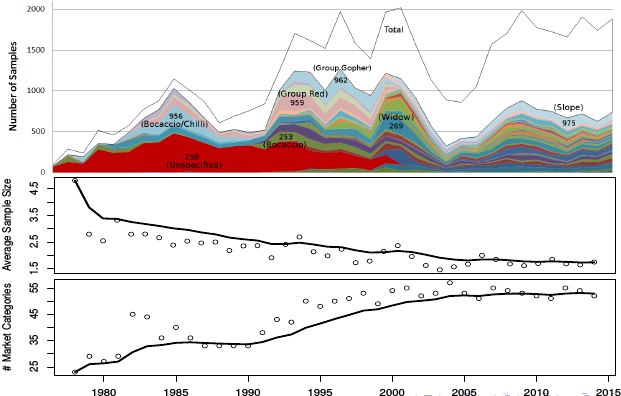
\includegraphics[width=0.8\textwidth]{sampleComplex.png}
        \caption{
                The $top$ $panel$ shows the total number of samples, from 1978 to 2015, in the major groundfish market categories.
                The $middle$ $panel$ shows the average sample size, per stratum, decreasing through time, as the number of market categories increases, over the same period, in the $bottom$ $panel$.
        }
\end{figure}

%
\begin{figure}[h!]
	\centering
        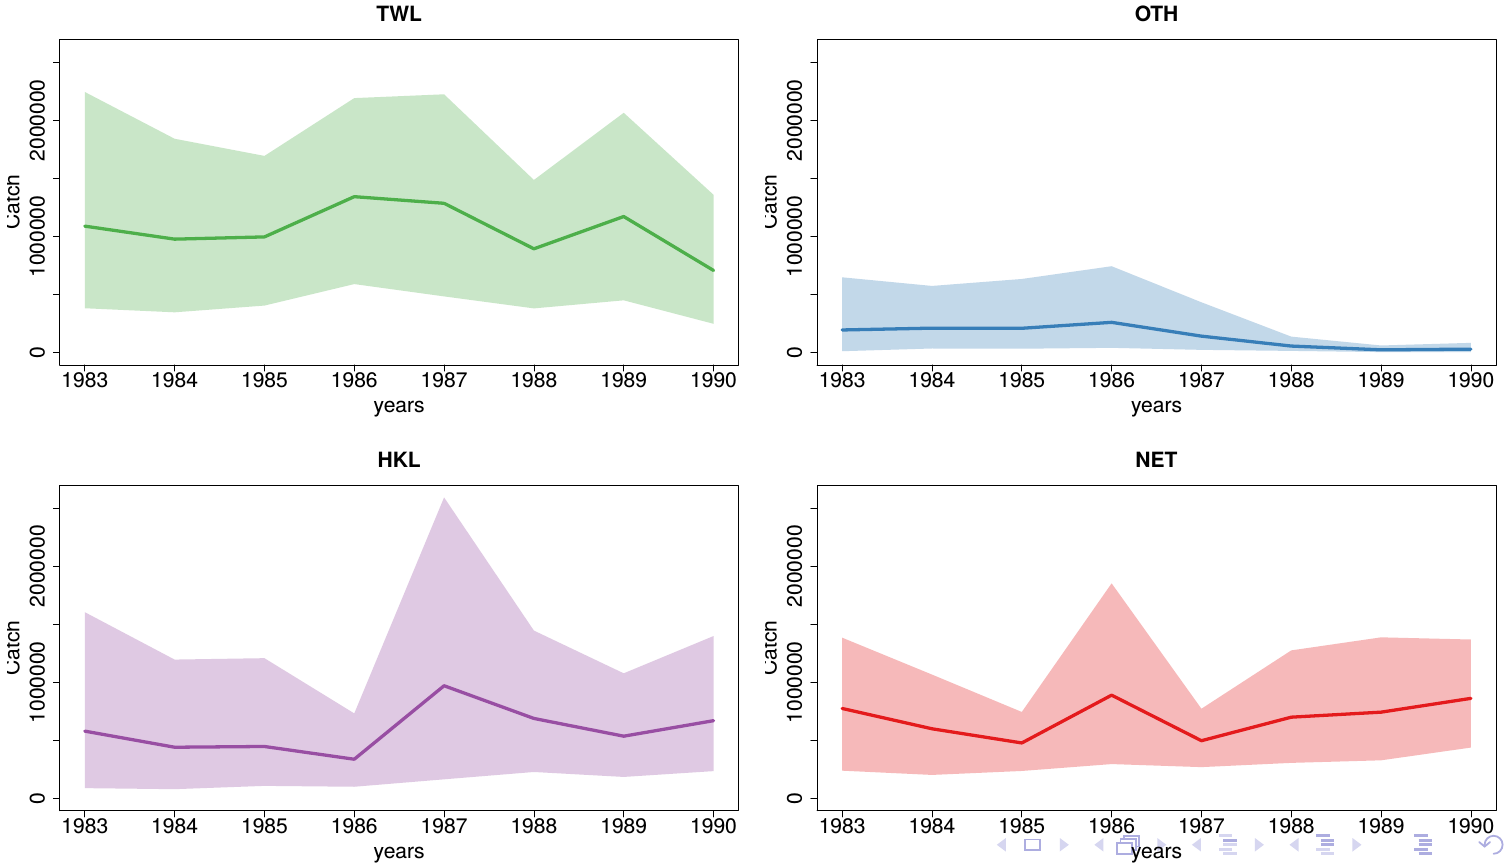
\includegraphics[width=0.9\textwidth]{./gearDists.png}
	\caption{Predicted landings distributions for Boccaccio through time, by gear.}
	%\hspace*{-0.6cm}  %0.59
        %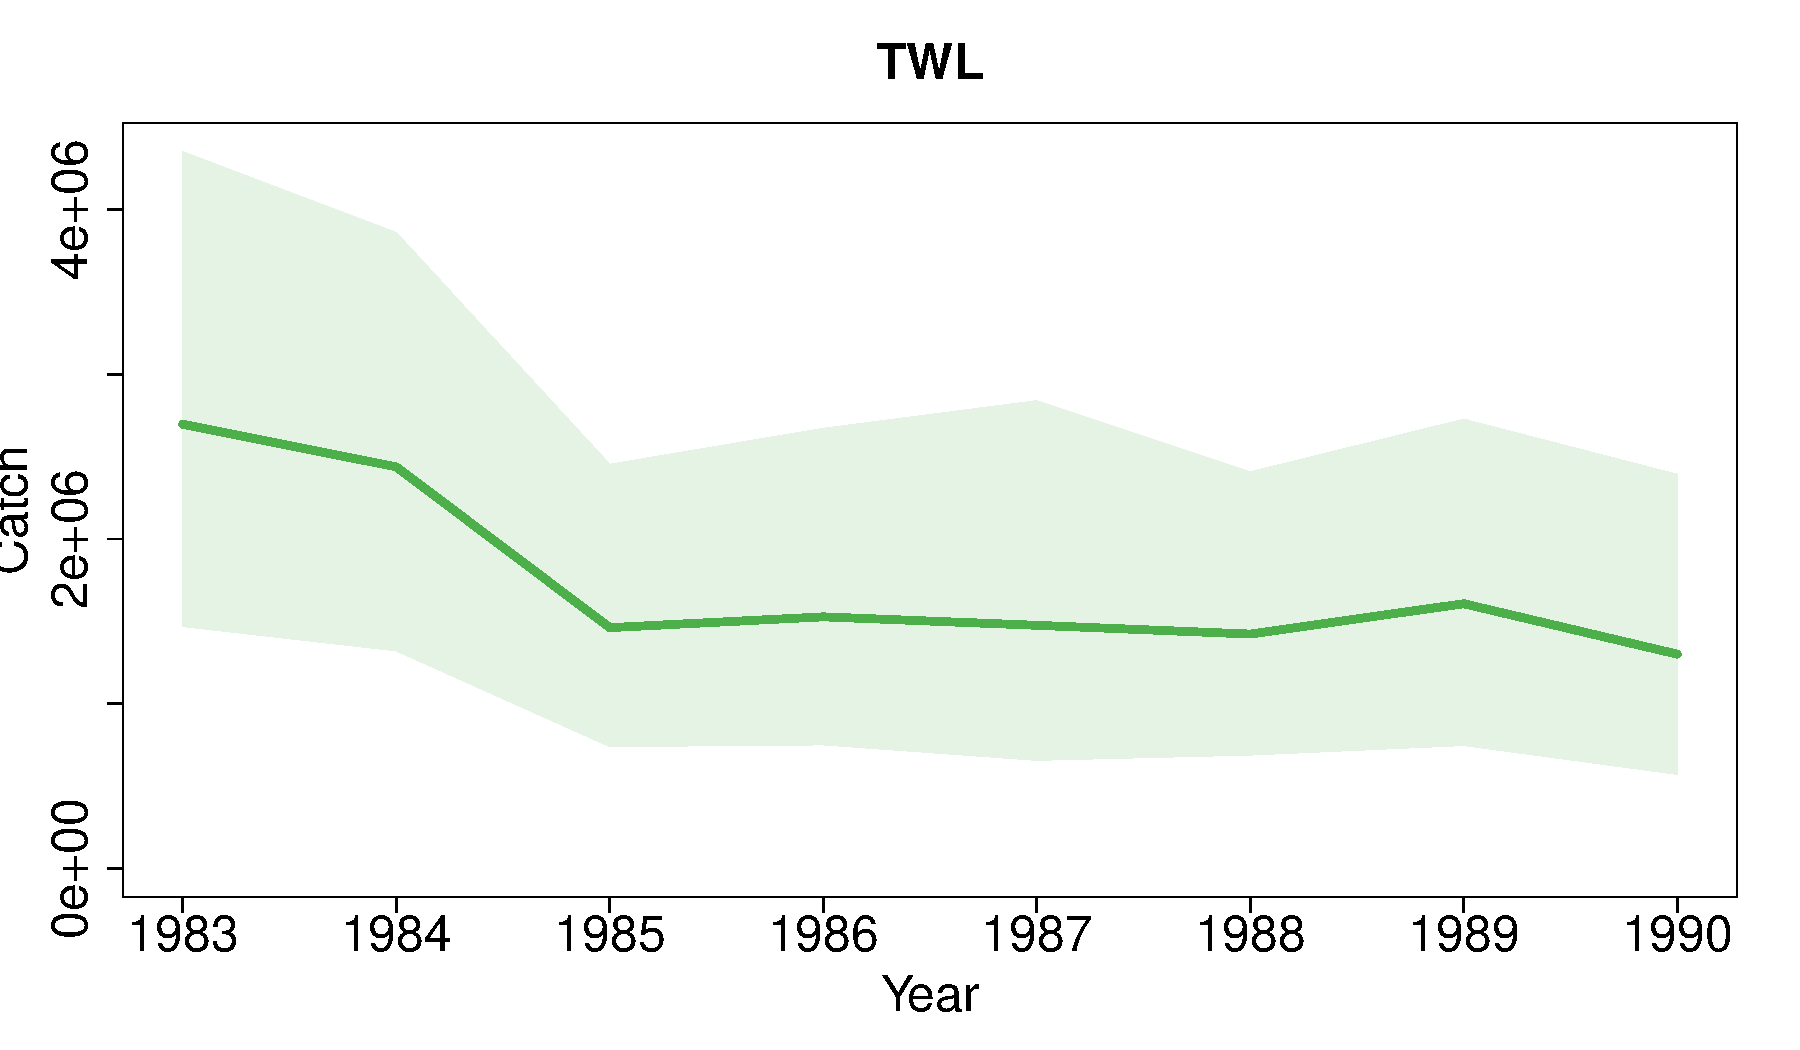
\includegraphics[width=0.55\textwidth]{./TWLLine.pdf}
        %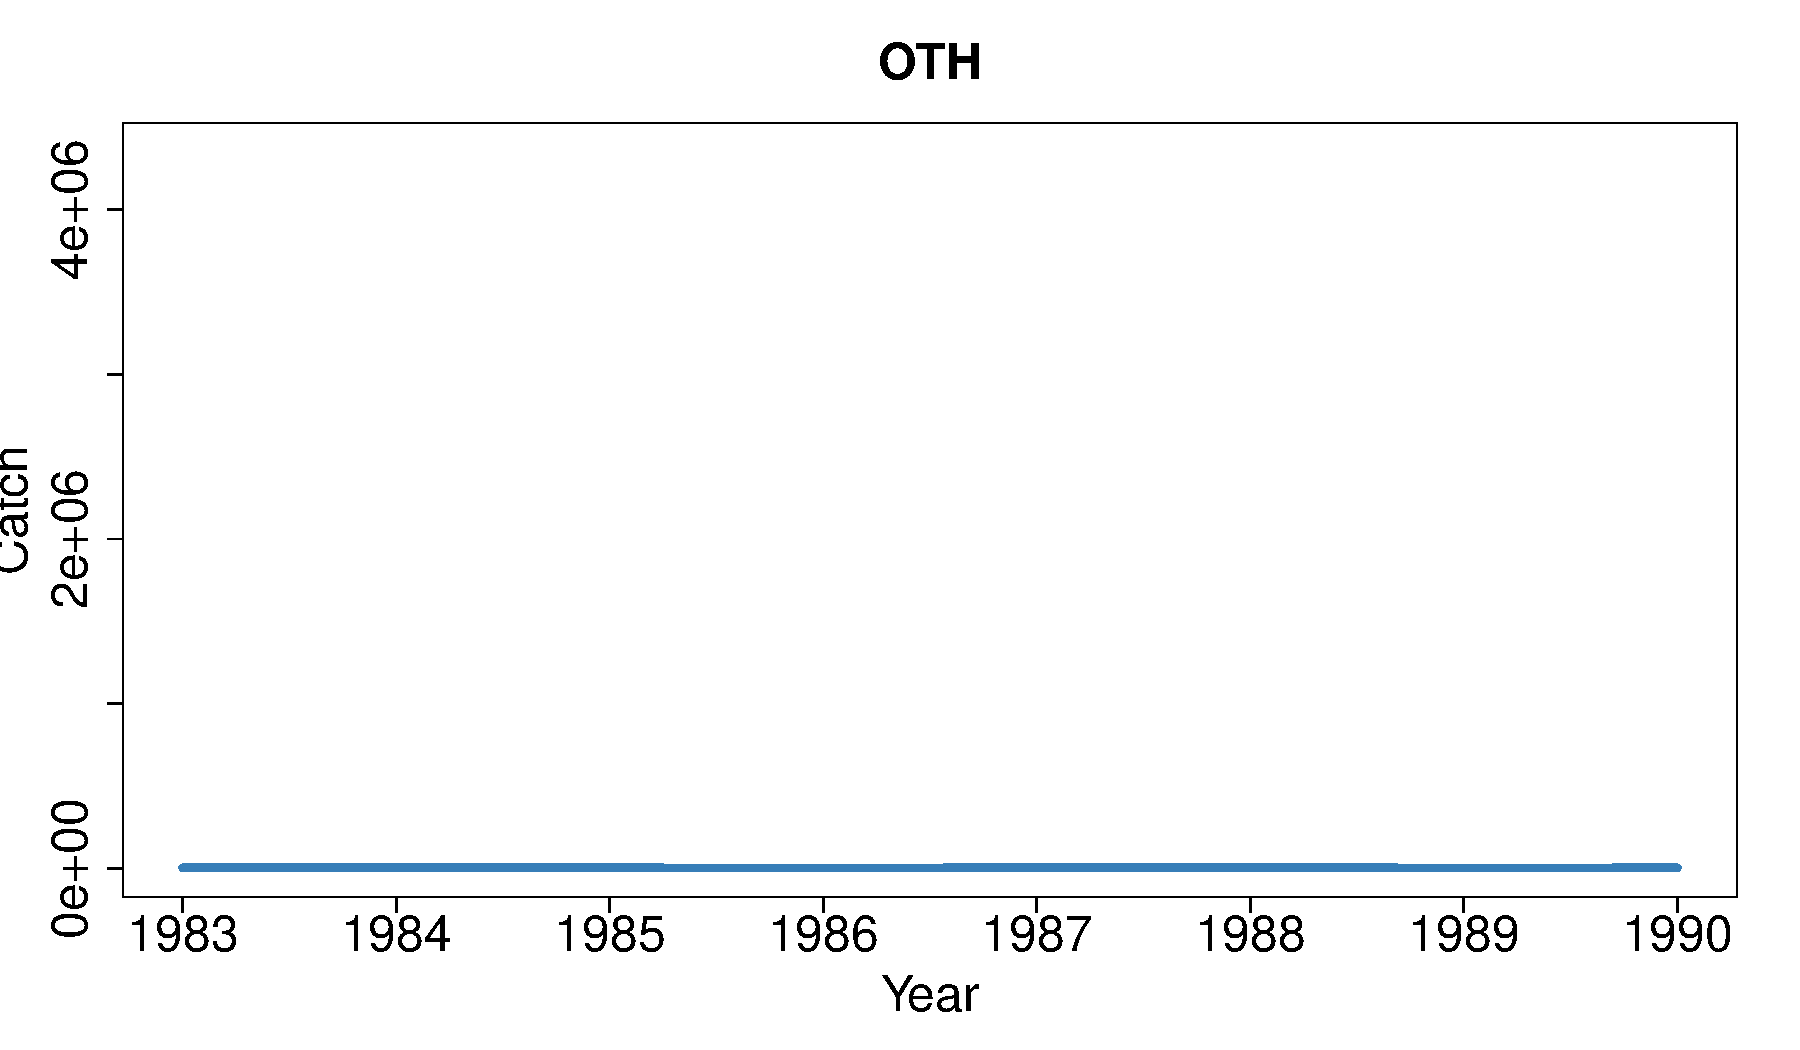
\includegraphics[width=0.55\textwidth]{./OTHLine.pdf}\\
        %\hspace*{-0.6cm}
        %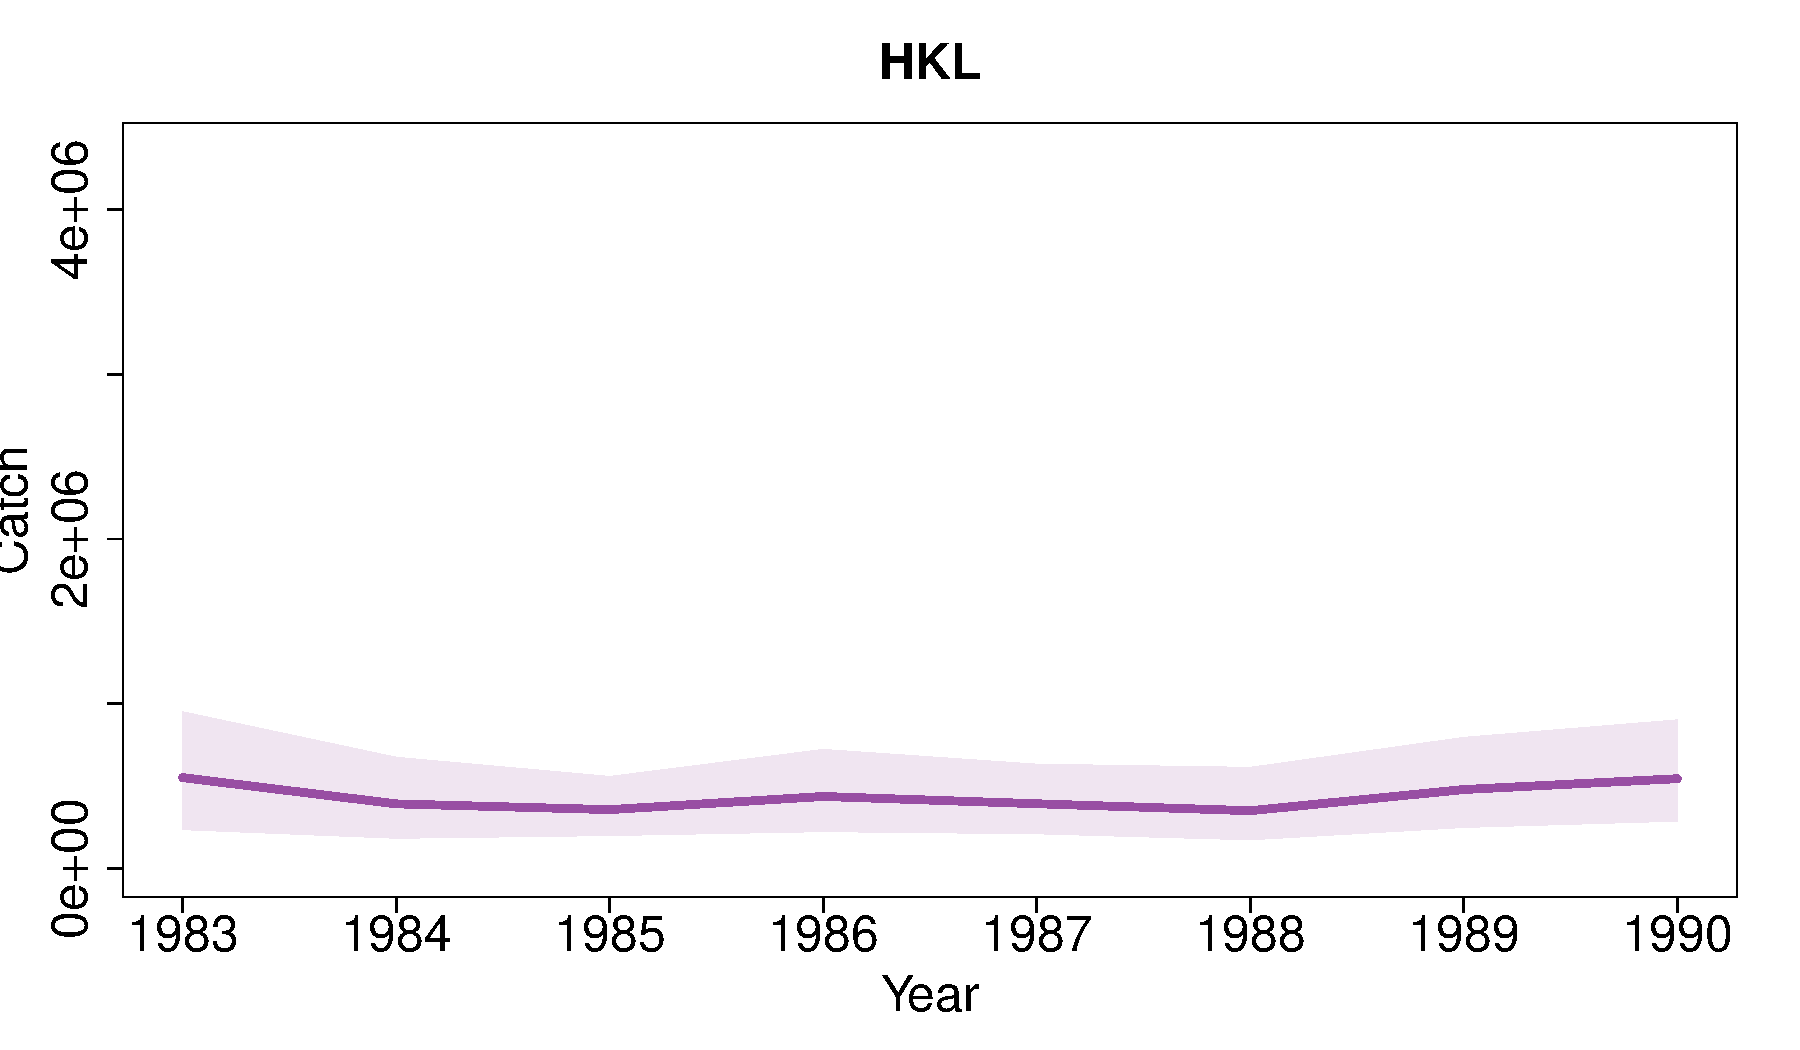
\includegraphics[width=0.55\textwidth]{./HKLLine.pdf}
        %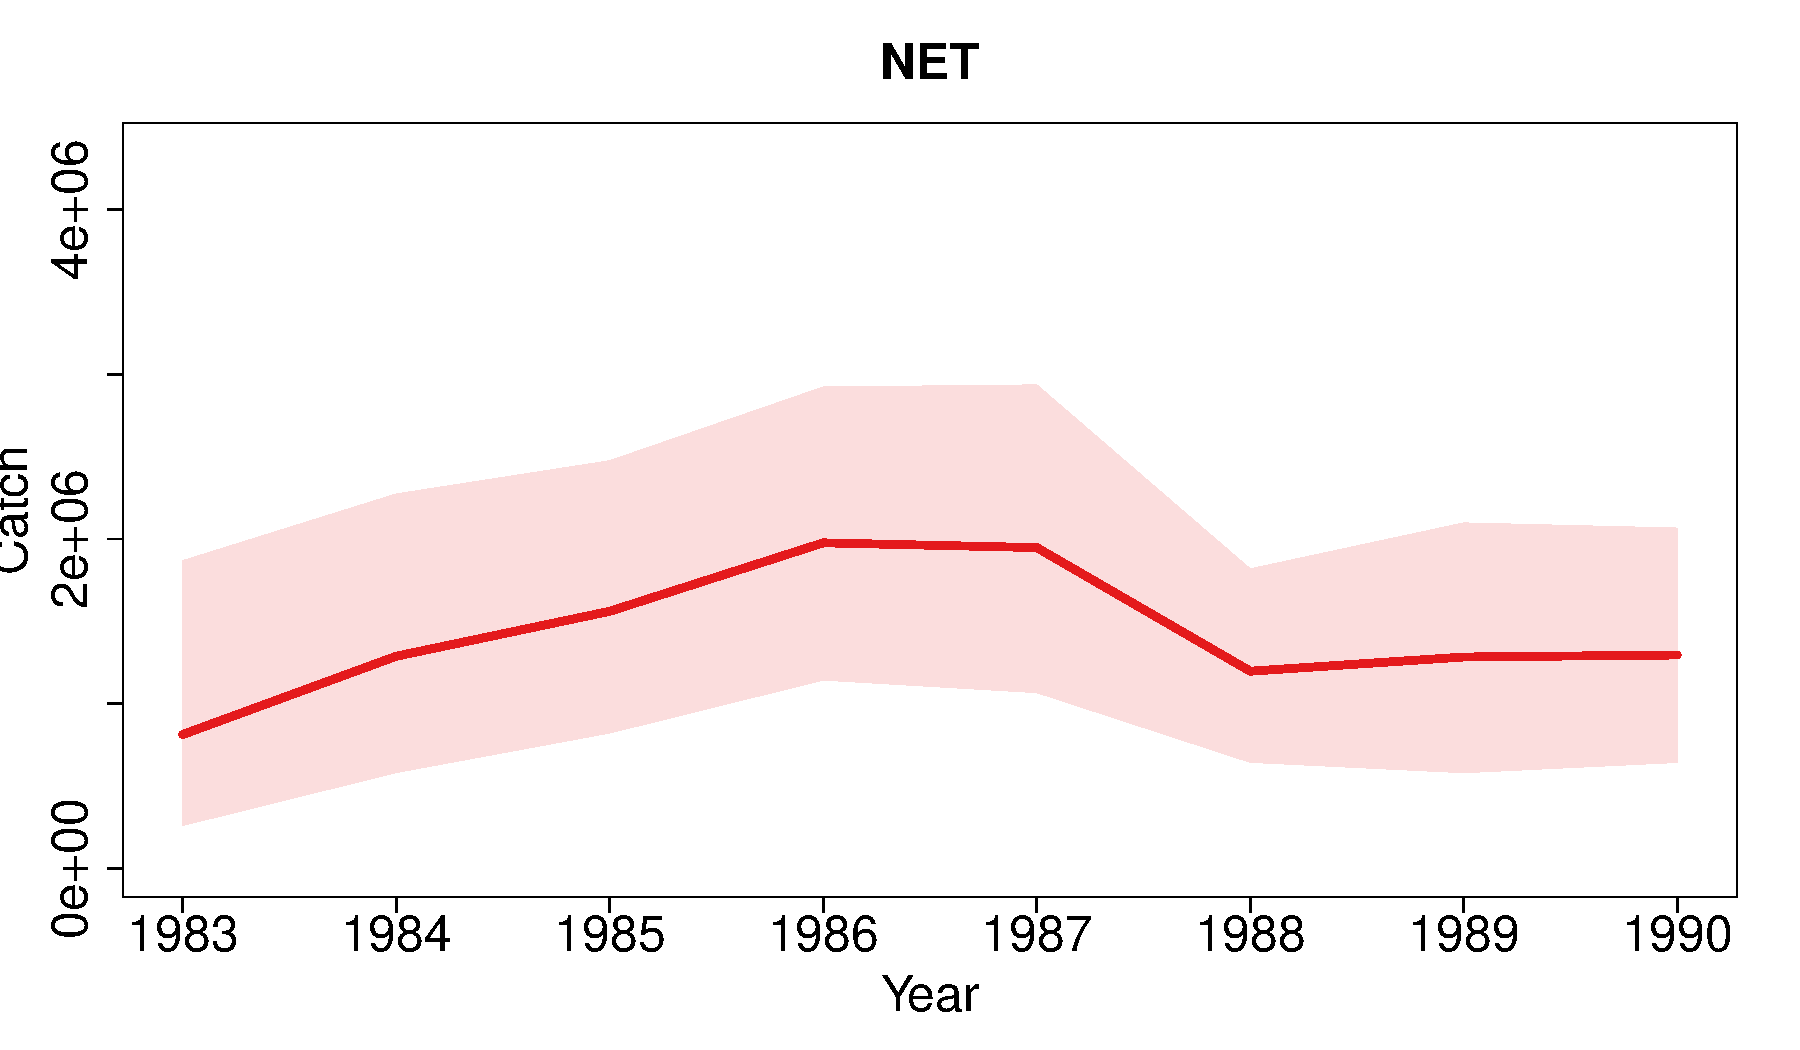
\includegraphics[width=0.55\textwidth]{./NETLine.pdf}
\end{figure}

%
\clearpage

%
%

%
\begin{thebibliography}{1}

%
\bibitem{gelman} Gelman, A., Carlin, J. B., Stern, H. S., \& Rubin, D. B.
(2014). Bayesian data analysis (Vol. 2). Boca Raton, FL, USA: Chapman \&
Hall/CRC.

%
\bibitem{bma} Hoeting, J. A., Madigan, D., Raftery, A. E., \& Volinsky, C. T.
(1999). Bayesian model averaging: a tutorial. Statistical science, 382-401.

%
\bibitem{pearsonErwin} Pearson, D.E., and Erwin, B. (1997). Documentation of
California’s commercial market sampling data entry and expansion programs.
NOAA Tech Memo. NOAA-TM-NMFS-SWFSC-240.

%
\bibitem{rCoreTeam} R Core Team (2015). R: A language and environment for
statistical computing. R Foundation for Statistical Computing, Vienna,
Austria. URL https://www.R-project.org/.

%
\bibitem{inlaPackage} Rue H., Martino S., Lindgren F., Simpson D., Riebler A.
(2013). R-INLA: Approximate Bayesian Inference using Integrated NestedLaplace
Approximations. Trondheim, Norway. URL http://www.r-inla.org/.

%
\bibitem{inlaMethod} Rue, H., Martino, S., \& Chopin, N. (2009). Approximate
Bayesian inference for latent Gaussian models by using integrated nested Laplace
approximations. Journal of the royal statistical society: Series b
(statistical methodology), 71(2), 319-392.

%
\bibitem{senMemo} Sen, A.R. (1984). Sampling commercial rockfish landings in
California. NOAA Tech Memo. NOAA-TM-NMFS-SWFSC-45.

%
\bibitem{senPaper} Sen AR. (1986). Methodological problems in sampling
commercial rockfish landings. Fish Bull. 84: 409-421 .

%
\bibitem{sheltonEtAl} Shelton, A. O., Dick, E. J., Pearson, D. E., Ralston,
S., \& Mangel, M. (2012). Estimating species composition and quantifying
uncertainty in multispecies fisheries: hierarchical Bayesian models for
stratified sampling protocols with missing data. Canadian Journal of Fisheries
and Aquatic Sciences, 69(2), 231-246.

\end{thebibliography}

%
\end{document}

